\chapter{Supports, exécution et signes}\label{ch:supports}

Les notices issues de l’EDCS ne contenaient aucune donnée matérielle : ni support, ni matériau, ni dimensions, ni signes figurés. Les fiches EpiDoc de l’EDB en fournissent pour \st{edbXmlC} des \st{nC} textes funéraires. Ces descriptions sont celles des rédacteurs de la base, nommés dans chaque notice ; elles reposent sur l’édition, sur les photographies et, pour une partie des pierres, sur l’autopsie de l’équipe de Bari. Elles n’ont pas été contrôlées ici et doivent être lues comme des données transmises.

\section{Supports, matériaux et techniques}

% généré par scripts/04_generated.py
\begin{table}[tbp]\centering\small\caption{Support, matériau et technique d’exécution selon les fiches EpiDoc de l’EDB (ensemble C ; 429 fiches).}\label{tab:supports}
\begin{tabular}[t]{@{}l r@{}}\toprule Support & N\\\midrule plaque & 349\\ non précisé & 53\\ sarcophage & 12\\ enduit de mortier & 11\\ paroi & 3\\ brique & 1\\\bottomrule\end{tabular}\hspace{1.2em}\begin{tabular}[t]{@{}l r@{}}\toprule Matériau & N\\\midrule marbre & 361\\ non précisé & 53\\ mortier & 11\\ enduit & 3\\ maçonnerie de briques & 1\\\bottomrule\end{tabular}\hspace{1.2em}\begin{tabular}[t]{@{}l r@{}}\toprule Exécution & N\\\midrule gravée & 360\\ non précisé & 54\\ tracée dans le mortier frais & 11\\ peinte & 3\\ graffitée & 1\\\bottomrule\end{tabular}\end{table}


La plaque de marbre domine très largement (tableau~\ref{tab:supports}). C’est le support ordinaire de la fermeture d’un \emph{loculus} ou d’une tombe à formes dans les catacombes et dans les cimetières à ciel ouvert. Pour \st{nPlaquesMes} plaques dont les deux dimensions sont données, la hauteur médiane est de \st{medH}~cm et la largeur médiane de \st{medW}~cm ; les largeurs s’étendent de \st{minW} à \st{maxW}~cm. Ces mesures ne disent rien de l’état complet du monument : une partie des plaques est fragmentaire.

Trois autres groupes, plus petits, méritent l’attention.

\emph{Les sarcophages} (\st{nSarco} textes : \nnums{\st{sarcolist}}). Le texte est alors gravé sur la cuve ou le couvercle d’un monument coûteux. Plusieurs de ces textes figurent parmi les plus longs et les plus élaborés du corpus : le poème de Maximilla et la notice de Lucceia (\nnum{306}, 72 × 212 cm, Platonia de Saint-Sébastien), l’épitaphe métrique de Felicitas (\nnum{470}), l’épitaphe de Cassia, \emph{clarissima femina} (\nnum{15}).

\emph{Les inscriptions tracées dans le mortier frais} (\st{nMortier} textes : \nnums{\st{mortierlist}}). Le texte est incisé au moment de la fermeture de la tombe, dans l’enduit qui scelle le \emph{loculus}. Ces inscriptions sont souvent brèves ; l’une d’elles (\nnum{311}) porte la formule \emph{in Chr(isto)} et un chrisme.

\emph{Les inscriptions peintes et graffitées} (\nnums{\st{peinteslist}} pour la peinture, 325 pour le graffite sur brique). L’inscription peinte du \nnum{206} est celle pour laquelle l’EDB donne une date (377) incompatible avec la formule consulaire (370) : la date de la base est vraisemblablement fautive.

L’EDB qualifie de métriques dix textes (\nnums{\st{metrlist}}). Cette qualification est incomplète : d’autres textes du corpus sont métriques ou rythmés (par exemple le \nnum{306}, que l’EDB ne qualifie pas ainsi, ou le \nnum{352}, recueilli dans les \emph{Carmina Latina Epigraphica}). Elle ne peut servir à mesurer la part des épitaphes en vers.

\section{Reproductions disponibles}

L’EDB signale une reproduction pour \st{nFacsim} textes funéraires : photographies de la Pontificia Commissione di Archeologia Sacra, dessins de l’ICVR I de De Rossi, reproductions tirées de publications (Perret 1851, ICVR IV, corpus régionaux). Ces images sont protégées (« Rights Reserved — Free Access via Epigraphic Database Bari ») ; elles n’ont pas été reproduites. Leur existence est signalée dans chaque notice, car elle définit le programme d’un contrôle photographique.

\section{Les signes chrétiens}

\subsection{Un marquage invisible dans la première base}

L’EDB décrit des chrismes et des croix sur \st{nSignesA} textes du catalogue, dont \st{nSignesC} textes funéraires, soit \st{pSignesC}~\% des \st{edbAppC} textes funéraires appariés. L’EDCS n’en signale aucun, sauf au \nnum{38}, où le monogramme est rendu par un mot développé. Ce chiffre est un minimum : les textes tronqués des listes de résultats peuvent omettre un signe placé en fin de texte, et les fiches EpiDoc de 2019 ne décrivent pas toujours le décor. Il dépend aussi de la description de l’EDB, qui n’a pas été vérifiée sur photographie.

\begin{table}[tbp]\centering\small
\caption{Types de signes décrits par l’EDB (ensemble C ; un texte peut porter plusieurs signes).}\label{tab:typessignes}
\begin{tabular}{@{}l r@{}}\toprule Signe & Textes\\\midrule
chrisme & 49\\ chrisme avec alpha et oméga & 23\\ croix monogrammatique & 10\\ croix monogrammatique avec alpha et oméga & 5\\ croix & 2\\ chrisme radié, alpha et oméga seuls, croix gammée & 1 chacun\\\bottomrule
\end{tabular}
\end{table}

Le chrisme, simple ou accompagné de l’alpha et de l’oméga, domine (tableau~\ref{tab:typessignes}). La croix monogrammatique, où la haste du P se combine avec une croix, apparaît plus rarement. L’EDB décrit en outre des signes qui ne sont pas comptés ici comme christiques : oiseaux, palmes, feuilles, couronnes, orants.

\subsection{Une part qui décroît}

Rapportée aux textes appariés de chaque période, la part des textes portant un chrisme ou une croix décroît : environ un texte sur quatre dans les années 340–359, un sur dix dans les années 390–403 (tableau~\ref{tab:signesper}, figure~\ref{fig:signes}). Cette tendance doit être interprétée avec prudence. Elle peut traduire un changement des pratiques de gravure ; elle peut aussi tenir à la composition topographique du corpus, qui change avec le temps (chapitre~\ref{ch:provenance}), ou à l’inégale description du décor selon les secteurs et les rédacteurs de la base. Elle n’autorise aucune conclusion sur l’intensité de l’identité chrétienne.

% généré par scripts/04_generated.py
\begin{table}[tbp]\centering\small\caption{Textes de l’ensemble C portant un chrisme ou une croix selon l’EDB, par période, rapportés aux textes appariés à une fiche EDB.}\label{tab:signesper}
\begin{tabular}{@{}l r r r@{}}\toprule Période & Signes & Textes appariés & \%\\\midrule
340–359 & 12 & 50 & 24,0 \\
360–374 & 24 & 114 & 21,1 \\
375–389 & 16 & 132 & 12,1 \\
390–403 & 15 & 147 & 10,2 \\
\bottomrule\end{tabular}\end{table}


\begin{figure}[tbp]\centering
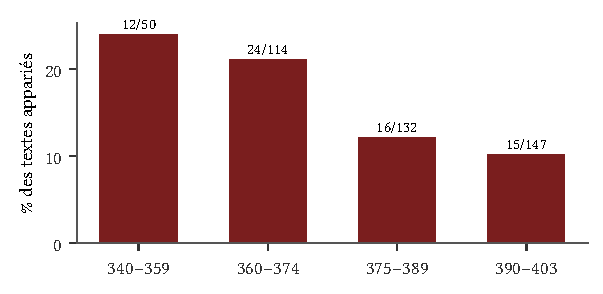
\includegraphics[width=0.62\linewidth]{figures/fig_signes.pdf}
\caption{Part des textes funéraires appariés portant un chrisme ou une croix selon l’EDB, par période.}\label{fig:signes}
\end{figure}

\subsection{Signes et formulaire}

Les textes qui portent un signe sont plus souvent pourvus de la formule \emph{in pace} que les autres : \st{ipSigne} contre \st{ipSansSigne}. L’association est nette, mais elle ne démontre pas une relation de sens. Les textes à signe décrit sont aussi, en moyenne, mieux conservés et mieux documentés ; et le signe, comme la formule, appartient à un même registre de marquage chrétien du monument. La mesure montre seulement que signe et formule ne se substituent pas l’un à l’autre : ils se cumulent.

\subsection{Quand le signe tient lieu de mot}

Dans quatre textes, la question du signe touche directement le vocabulaire. Au \nnum{38}, l’EDB transcrit \emph{in pace ((monogramma Christi))} là où l’EDCS donne \emph{in pace Chr(isti)}, et l’estampage universitaire montre un christogramme après IN PACE. Aux \nnums{140} et 151 (\emph{in pace Chr(isti)}) et au \nnum{311} (\emph{in Chr(isto)}), les deux bases transcrivent un mot abrégé, mais l’EDB décrit un chrisme sur le support. Il est probable que, dans ces trois textes, l’abréviation développée rende un monogramme employé comme compendium du nom du Christ ; il n’est pas exclu qu’elle coexiste avec un chrisme décoratif distinct. Les deux bases, et sans doute les éditeurs qu’elles suivent, ont fait des choix de transcription différents pour des situations peut-être identiques. La conséquence est traitée au chapitre~\ref{ch:dieu_christ} : ces quatre textes ne peuvent être comptés comme des mentions écrites du Christ sans contrôle des photographies.

% généré par scripts/04_generated.py
\begin{longtable}{@{}r r p{0.7\linewidth}@{}}\caption{Signes chrétiens décrits par l’EDB (fiches EpiDoc de 2019 et texte des listes de résultats de 2026), ensemble A.}\label{tab:signes}\\\toprule N° & Année & Signes\\\midrule\endfirsthead\toprule N° & Année & Signes\\\midrule\endhead\bottomrule\endfoot
4 & 341 & chrisme \\
9 & 343 & chrisme \\
16 & 346 & chrisme \\
22 & 348 & chrisme et chrisme radié \\
24 & 348 & croix \\
34 & 350 & chrisme \\
38 & 352 & chrisme \\
43 & 355 & chrisme et chrisme avec alpha et oméga \\
46 & 356 & chrisme \\
49 & 358 & chrisme \\
50 & 358 & chrisme \\
55 & 359 & chrisme et chrisme avec alpha et oméga \\
60 & 361 & chrisme \\
61 & 361 & chrisme \\
68 & 362 & chrisme et chrisme avec alpha et oméga \\
73 & 363 & alpha et oméga, chrisme, croix et croix gammée \\
94 & 365 & chrisme \\
95 & 365 & croix monogrammatique avec alpha et oméga \\
99 & 366 & chrisme \\
100 & 366 & chrisme \\
106 & 367 & chrisme \\
109 & 367 & chrisme et chrisme avec alpha et oméga \\
118 & 367 & chrisme \\
120 & 367 & chrisme \\
124 & 367 & chrisme \\
128 & 368 & chrisme \\
136 & 370 & chrisme et chrisme avec alpha et oméga \\
139 & 370 & chrisme \\
140 & 370 & chrisme \\
142 & 370 & chrisme \\
143 & 371 & chrisme et chrisme avec alpha et oméga \\
146 & 371 & chrisme et chrisme avec alpha et oméga \\
147 & 371 & chrisme \\
151 & 371 & chrisme \\
160 & 372 & chrisme avec alpha et oméga \\
168 & 373 & croix monogrammatique \\
175 & 374 & chrisme avec alpha et oméga \\
179 & 375 & chrisme et chrisme avec alpha et oméga \\
183 & 375 & chrisme \\
185 & 375 & chrisme avec alpha et oméga \\
186 & 375 & chrisme \\
191 & 376 & chrisme \\
193 & 376 & chrisme et chrisme avec alpha et oméga \\
209 & 378 & chrisme et chrisme avec alpha et oméga \\
213 & 380 & chrisme et croix monogrammatique \\
225 & 381 & chrisme avec alpha et oméga \\
247 & 383 & chrisme \\
260 & 384 & chrisme et chrisme avec alpha et oméga \\
273 & 384 & chrisme et chrisme avec alpha et oméga \\
275 & 385 & chrisme et chrisme avec alpha et oméga \\
276 & 385 & chrisme \\
300 & 388 & croix monogrammatique avec alpha et oméga \\
304 & 389 & chrisme et chrisme avec alpha et oméga \\
311 & 388 & chrisme \\
321 & 390 & chrisme \\
324 & 390 & chrisme avec alpha et oméga \\
344 & 392 & croix monogrammatique et croix monogrammatique avec alpha et oméga \\
348 & 392 & croix monogrammatique \\
349 & 392 & chrisme avec alpha et oméga \\
357 & 393 & croix monogrammatique \\
369 & 395 & croix monogrammatique \\
376 & 395 & chrisme, chrisme avec alpha et oméga, croix monogrammatique et croix monogrammatique avec alpha et oméga \\
400 & 397 & chrisme et croix monogrammatique \\
402 & 397 & croix monogrammatique \\
430 & 399 & croix monogrammatique \\
431 & 399 & chrisme et chrisme avec alpha et oméga \\
434 & 397 & chrisme et chrisme avec alpha et oméga \\
453 & 401 & chrisme avec alpha et oméga \\
454 & 401 & croix monogrammatique avec alpha et oméga \\
465 & 402 & chrisme \\
\end{longtable}

